\chapter{Experimentos y resultados}\label{chapter:experiments}
% Revisión 2026-11-07: declaraciones del autor en fix.md; artefactos y hashes en
% ../tablas/revision.json. Los informes del piloto anterior conservan su alcance histórico.
% Validaciones del generador: docs/resumen.md y Evaluations/estudio/lecturas/.

Este capítulo presenta las \textbf{Condiciones y el corpus} (Sección~\ref{sec:corpus}), las
\textbf{Validaciones del generador} (Sección~\ref{sec:validaciones}), la \textbf{Validación del
extractor} (Sección~\ref{sec:resultados-extractor}) y el \textbf{Análisis horizontal}
(Sección~\ref{sec:resultados-horizontal}). Después describe el \textbf{Estudio humano}
(Sección~\ref{sec:resultados-estudio}), el \textbf{Juez aprendido}
(Sección~\ref{sec:resultados-juez}) y la \textbf{Ordenación del corpus}
(Sección~\ref{sec:resultados-ranking}). Cierra con la \textbf{Respuesta a las hipótesis}
(Sección~\ref{sec:respuesta-hipotesis}). Se distingue entre los resultados reconstruibles desde los
artefactos y la información del estudio actualizada por el autor el 7 de noviembre de 2026; los
recuentos de participación proceden de esta última.

\section{Condiciones y corpus}\label{sec:corpus}

Todas las historias de este capítulo se generaron con la API de Gemini, sujeta a la cuota diaria
descrita en la Sección~\ref{sec:proveedores}, y con los dos modelos de la configuración de ejemplo:
\texttt{gemini-3.5-flash-lite} como modelo principal y \texttt{gemini-3.1-flash-lite} para los turnos
y las reflexiones de los actores, según los modelos que registra cada ejecución. El extractor de
rasgos usó \texttt{gemini-3.5-flash-lite}. Los contrastes de generación documentados mantienen la versión del
generador y la entrada: los cambios de narración, sobre la misma función, y los de
escritura, sobre el mismo plan (Sección~\ref{sec:artefactos}).

El corpus es el conjunto de ejecuciones guardadas en la copia del autor del repositorio, en la
carpeta \texttt{Stories/}, que no está bajo control de versiones (Sección~\ref{sec:pruebas}). El
inventario del 28
de octubre de 2026, hecho con \texttt{asg-corpus} antes de generar la matriz, contó 331 ejecuciones,
de las que 116 eran elegibles para el ranking: las completas y en prosa de Stagecraft 7 y las líneas
base. Se excluyeron 135 por ser de un generador anterior a Stagecraft 7, 72 por no haber terminado y
8 por tener un formato fuera del estudio en prosa, como los guiones; ninguna se borró ni se editó a
mano. El 1 de noviembre de 2026, con la matriz ya generada, el mismo inventario cuenta 346
ejecuciones y 130 elegibles: 70 simuladas, 48 narrativas y 12 líneas base. De ellas, 26 son de la
versión de referencia (13 simuladas, 4 narrativas y 9 líneas base); las demás, de versiones anteriores de
Stagecraft 7, son elegibles según ese inventario. Este inventario histórico no identifica por sí
solo el corpus de 122 historias destinado a la ordenación en el estudio actualizado
(Sección~\ref{sec:resultados-ranking}).

Los experimentos usan tres obras del catálogo de siete peticiones preparado para ellos: una fantasía
canónica con un caballero, una princesa y un dragón (obra 01), un misterio, «La última luz del faro»
(obra 03), y un drama, «El cine de los domingos» (obra 04); sus peticiones están en el
Anexo~\ref{app:obras}. Sus líneas base de un solo
\textit{prompt} se generaron el 28 de octubre de 2026 con la versión de referencia: tres por obra, con la
variante Esencial literal del catálogo, la misma petición que recibe el generador, sin plan ni
revisión. Las nueve terminaron con una llamada cada una, salvo una que repitió tras un fallo del
proveedor. Su extensión va de 834 a 978 palabras en la obra 01, de 1.149 a 1.725 en la 03 y de 1.097
a 1.722 en la 04. Las tres repeticiones de cada obra estaban pensadas para medir el ruido de la
propia línea base (Sección~\ref{sec:horizontal}).

\section{Validaciones del generador}\label{sec:validaciones}

Los mecanismos con alternativa se probaron en ejecuciones reales y en sesiones de lectura.
Las comprobaciones técnicas y las sesiones conservadas del 27 de octubre documentan la elección de
la configuración de referencia de la Tabla~\ref{tab:mecanismos}. El autor informa además de otras
lecturas realizadas por participantes del estudio; sus respuestas no se agregan a las sesiones
conservadas sin un registro que permita identificar cada comparación. A continuación se presentan
las mediciones fechadas que pueden reconstruirse.

\subsection{El modo de la función}\label{sec:val-modo}

El 30 de septiembre de 2026, con la versión 7.5, dos funciones se representaron desde el mismo plan
de «La sombra del volcán», con el mismo presupuesto de turnos. En modo fijo, la función completó 6
escenas y 48 turnos, y de sus 6 \textit{beats} alcanzó 5 y forzó 1. En modo adaptativo terminó con un
cierre abierto tras 2 escenas y 16 turnos, con 1 de sus 2 \textit{beats} alcanzado. Ninguna cumplió
las dos promesas del plan. El modo fijo quedó como predeterminado y el adaptativo, como opción sin
lectura a ciegas. Son dos observaciones de una sola premisa: muestran que el modo adaptativo puede
cerrar la obra antes de tiempo, no cuál de los dos da mejores historias.

En esa validación se auditaron literalmente 62 contextos enviados a los actores, y ninguno contenía un
pensamiento de otro personaje ni un susurro que el actor no hubiera presenciado. Es la comprobación,
en ejecuciones reales, de lo que una prueba de contrato comprueba con el proveedor falso
(Sección~\ref{sec:pruebas}). No se conserva una tabla de esa auditoría, solo su resultado en
\texttt{docs/resumen.md}. Revisó dos categorías que el diseño ya mantiene privadas por construcción,
y con la versión 7.5, anterior a la referencia experimental. Para el contraste entre memorias es evidencia indirecta: es coherente con que la
memoria propia aísle a los personajes de esas dos fugas, pero no muestra que mejore las escenas.

\subsection{Narración y escritura}\label{sec:val-brazos}

El 27 de octubre de 2026, con la versión 7.21, se conservaron dos sesiones de lectura a ciegas de los brazos de
narración y de escritura de la Sección~\ref{sec:opcionales}. En la primera, cinco funciones ya
representadas se narraron de nuevo dos veces cada una: con la narración resumida (brazo A) y con la
narración por selección, el editor por fragmentos y los ejemplos de estilo (brazo B). En la segunda,
dos planes nuevos se escribieron en prosa directa dos veces por brazo: sin brazos (A) y con las
fichas de escena, el crítico con cita, el editor y los ejemplos (B). El autor leyó los pares en la
vista de lectura ciega de StageCraft (Sección~\ref{sec:interfaces}), sin saber qué brazo había
producido cada historia. La Tabla~\ref{tab:lecturas} resume lo que cambió en las medidas y lo que
eligió el lector.

\begin{table}[htb]
  \centering
  \caption{Sesiones documentadas de narración y escritura (autor, 2026-10-27)}
  \label{tab:lecturas}
  \small
  \begin{tabular}{@{}>{\raggedright\arraybackslash}p{2.2cm}>{\raggedright\arraybackslash}p{1.0cm}%
      >{\raggedright\arraybackslash}p{8.0cm}>{\raggedright\arraybackslash}p{2.2cm}@{}}
    \toprule
    Lectura & Pares & Medidas, brazo A frente a brazo B & Elección \\
    \midrule
    Narración de la función & 5 & réplicas con verbo de habla: 30--62~\% frente a 3--22~\%; párrafos
      con más de dos réplicas indirectas: de 1 a 6 por historia frente a ninguno en cuatro pares y 2
      en el quinto & A 2, B 2, ninguna 1 \\
    Escritura narrativa & 4 & proporción de réplicas con coletilla emocional: 0,00--0,21 frente a
      0,00; proporción de párrafos marcados por el código: 0,25--0,68 frente a 0,00--0,10; palabras:
      1.581--1.827 frente a 1.197--1.503 & A 3, B 1 \\
    \bottomrule
  \end{tabular}
\end{table}

En las dos lecturas, el brazo B corrigió los defectos medidos, y en ninguna ganó. En la narración, B
redujo los párrafos que encadenan réplicas en estilo indirecto, como un acta, y el verbo de habla en
casi cada línea, y empató con A. Estas dos cifras son aproximadas: salen de expresiones regulares y no
del código del repositorio. \texttt{docs/resumen.md} registra además dos medidas en contra de B. La
proporción de réplicas del registro que sobreviven en la narración, que calcula el código del
generador, fue de 0,73 a 0,85 frente a 0,48 a 0,67 de A. Las réplicas directas por ejecución fueron
de 18 a 68 frente a 12 a 35. B conservó, por tanto, más del registro tal cual, que es el riesgo de la
Sección~\ref{sec:narrador}. En la escritura, los ocho borradores ya
cumplían, con o sin brazos, los cuatro umbrales con que el código mide la prosa (nombres repetidos,
coletillas emocionales, gerundios en la coletilla y símiles); B redujo las coletillas a casi cero y
acortó el texto, y el lector prefirió A en tres de los cuatro pares. Con un empate se mantuvo la
narración más barata, y en la escritura, la preferida: todos los brazos quedaron apagados, como
opciones.

Al día siguiente, dos ejecuciones con la versión 7.21 comprobaron, sin corregir nada, dos defectos
conocidos. El plan de una petición con ficha detallada («Las islas del cielo», perfil Expansiva)
dejó fuera dos cosas que pedía la ficha, la división de la tripulación y quién paga el coste de la
decisión final, y el revisor del plan lo aprobó sin notas: no comprueba cada giro pedido, una
limitación observada en una sola ejecución. En cambio, un guion de la obra 03 salió con nombres,
papeles y reparto en español, sin una palabra en inglés.

\subsection{La configuración de referencia}\label{sec:val-congelada}

El 28 de octubre de 2026, la versión 7.22 se validó con tres ejecuciones de la obra 03, perfil
Esencial, con los valores predeterminados y sin corregir nada: una narrativa, un guion nativo y una
simulada. Las tres terminaron completas y con nombres en español. La narrativa hizo 22 llamadas y el guion, 18. La simulada hizo 236:
133 al modelo principal y 103 al de la función, 9 de ellas intentos fallidos que se repitieron, con
unos 570.000 \textit{tokens}. En la simulada se cumplieron todas las comprobaciones fijadas: los tres
capítulos salieron del narrador y no de un respaldo automático, ninguno de los 47 pensamientos de los
actores salió en inglés y ninguna línea de la historia quedó fuera de la ficción. Quedaron tres
defectos menores fuera de esos criterios en los textos conservados: una contracción omitida
(«de el faro») en la narrativa, un personaje de la ficha que el reparto del guion perdió y unos
títulos sin tilde en la simulada. Ese día se estableció la configuración de referencia para los experimentos, sin que ello
supusiera detener el desarrollo del generador.

La limitación conocida está en los \textit{beats}: la función forzó 3 de sus 6, en tres escenas
distintas. Es el precio del mecanismo de la Sección~\ref{sec:director}: el suceso del mundo garantiza
que la función avance, no que los personajes lleguen solos a cada evento. Las validaciones anteriores
no fijan la proporción: la de la versión 7.5 forzó 1 de 6 (Sección~\ref{sec:val-modo}), y
\texttt{docs/resumen.md} registra 5 de 10 en una de la 7.12, cuyos datos no se reproducen en esta
tesis. Con una ejecución, la cifra no separa el efecto del ruido.

Las sesiones documentadas muestran que reducir defectos medidos de la prosa no garantiza que el
lector prefiera el texto resultante: el brazo modificado empató en narración y perdió tres de los
cuatro pares de escritura. Esta observación es compatible con la hipótesis sobre los mecanismos
opcionales. Su alcance corresponde a esas sesiones; las lecturas adicionales requieren su propio
desglose para estimar cuánto se reproduce el resultado entre participantes.

\section{Validación del extractor}\label{sec:resultados-extractor}

La validación registrada el 29 de octubre de 2026 reúne doce historias: cinco simuladas con su
registro, cuatro narrativas y tres líneas base, de las versiones 7.8 a 7.22, con 21.471 palabras.
El modelo extractor fue \texttt{gemini-3.5-flash-lite}; en seis historias se repitió la extracción.
La Tabla~\ref{tab:extractor} reorganiza las hojas de revisión y el resumen de esas repeticiones.
Es una reconstrucción de los registros conservados, no una nueva revisión humana de las historias.

La precisión se calcula como ocurrencias correctas entre ocurrencias con veredicto correcto o
incorrecto. Las valoraciones sin resolución se mantienen fuera de ese denominador, conforme al
procedimiento de la Sección~\ref{sec:validacion-extractor}; sus recuentos se muestran en la
Tabla~\ref{tab:extractor-detalle} del Anexo~\ref{app:tablas}. Por ello, una precisión de 1,00 describe
las citas resueltas, no garantiza que se haya contado todo ni equivale a una validación completa.
Los campos de omisiones de las hojas están vacíos y no permiten calcular cobertura.

\begin{table}[p]
  \centering
  \caption{Validación registrada del extractor: citas y repetición (12 historias, 2026-10-29)}
  \label{tab:extractor}
  \small
  \setlength{\tabcolsep}{5pt}
  % Revisión documental 2026-11-07; fuentes en revision.json.
\begin{tabular}{@{}>{\raggedright\arraybackslash}p{5.1cm}rrrr@{}}
\toprule
Rasgo & \shortstack{Citas\\juzgadas} & Precisión & \shortstack{Pares\\comparables} & \shortstack{Diferencia\\media} \\
\midrule
Promesas de apertura & 5 & 1,00 & 5/6 & 0,00 \\
Señales de progreso & 15 & 1,00 & 4/6 & 0,00 \\
Preparación del pago final & 1 & 1,00 & 1/6 & 0,00 \\
Ciclos «sí, pero» & 5 & 1,00 & 2/6 & 0,00 \\
Ciclos «no, y además» & 5 & 1,00 & 2/6 & 0,25 \\
Proactividad del protagonista & 10 & 1,00 & 4/6 & 0,19 \\
Soluciones preparadas & 5 & 1,00 & 1/6 & 0,00 \\
Límites del mundo & 6 & 1,00 & 4/6 & 0,12 \\
Escenas con cambio & 7 & 1,00 & 2/6 & 0,00 \\
Decisiones con coste & 8 & 1,00 & 2/6 & 0,00 \\
Escenas con conflicto & 28 & 1,00 & 3/6 & 0,00 \\
Mentiras & 0 & --- & 1/6 & 0,00 \\
Secretos revelados & 3 & 1,00 & 3/6 & 0,00 \\
Complicaciones & 21 & 1,00 & 4/6 & 0,00 \\
Giros & 9 & 1,00 & 3/6 & 0,17 \\
Sucesos azarosos o externos & 6 & 1,00 & 4/6 & 0,18 \\
Usos de objetos & 21 & 1,00 & 4/6 & 0,22 \\
Contradicciones & 1 & 1,00 & 1/6 & 0,00 \\
\bottomrule
\end{tabular}

  \par\medskip
  \begin{minipage}{0.94\textwidth}
    \footnotesize
    Citas juzgadas: ocurrencias con veredicto resuelto; con menos de cinco, el apoyo es reducido.
    Pares comparables: historias con el rasgo medido en ambas extracciones, de seis repetidas.
    Diferencia media: promedio de $|a-b|/\max(|a|,|b|,1)$ sobre esos pares.
    El guion indica que no hay denominador; una diferencia nula no informa sobre las historias
    que no pudieron compararse.
  \end{minipage}
\end{table}
% Reconstrucción: verdict_summary(hojas/*.csv) y retest/resumen.json; hashes en revision.json.

La tabla presenta los dieciocho rasgos núcleo extraídos con citas. Los otros seis se calculan por
código: palabras, proporción de diálogo, repetición de trigramas, cuota del personaje más presente,
reparto de la participación y reparto del diálogo. Los tres últimos dependen de la segmentación o
las réplicas extraídas; por eso también se informa su repetibilidad en el anexo. Los cambios entre
los estados medido, no aplicable y fallido se separan allí de las diferencias numéricas.

La lista vigente contiene 24 rasgos núcleo. Los registros de validación corresponden al catálogo
anterior a esa selección; no se mezclan automáticamente con extracciones del catálogo vigente.
La presentación revisada conserva sus fechas y denominadores y permite identificar qué observaciones
necesitan una nueva revisión antes de atribuirles precisión o cobertura humana.

\section{Análisis horizontal}\label{sec:resultados-horizontal}

El conjunto presentado comprende \textbf{24 ejecuciones completadas}: cinco bases simuladas,
nueve líneas base de un solo \textit{prompt}, dos narrativas escritas desde el plan y ocho
renarraciones con cambios de tono o visión. Una unidad es una ejecución de una configuración para
una obra y una repetición determinadas; no es un rasgo ni una comparación. La
Tabla~\ref{tab:horizontal-conjunto} desglosa este conjunto y distingue la generación terminada de
la disponibilidad de una extracción núcleo completa y compatible.

\begin{table}[htb]
  \centering
  \caption{Conjunto horizontal y extracciones localizadas (revisión, 2026-11-07)}
  \label{tab:horizontal-conjunto}
  \small
  \setlength{\tabcolsep}{4pt}
  % Revisión documental 2026-11-07; fuentes en revision.json.
\begin{tabular}{@{}llrr@{}}
\toprule
Celda & Configuración & Ejecuciones & \shortstack{Extracción núcleo\\completa y compatible} \\
\midrule
M01 & Base simulada & 5 & 2 \\
M02 & Línea base de un prompt & 9 & 3 \\
M03 & Narrativa desde el plan & 2 & 0 \\
M04 & Tono sombrío & 2 & 2 \\
M05 & Tono humorístico & 2 & 0 \\
M06 & Visión limitada & 2 & 0 \\
M07 & Primera persona & 2 & 1 \\
 & Total & 24 & 8 \\
\bottomrule
\end{tabular}

\end{table}

Las líneas base y una base simulada proceden del 28 de octubre; las restantes ejecuciones se
completaron el 30 de octubre de 2026. El manifiesto, actualizado el 31 de octubre en UTC, contiene
45 posiciones históricas: las 24 completadas, una fallida y veinte pendientes. El
Anexo~\ref{app:tablas} conserva ese desglose. El total de 24 describe el conjunto final seleccionado
para este análisis, sin modificar retrospectivamente el diseño registrado.

La matriz reutiliza el plan o la función de una base: la escritura directa cambia el procedimiento
que produce la prosa, mientras que las variantes de tono y visión mantienen el registro de la
función. La Tabla~\ref{tab:coste} presenta el coste conservado por tipo de ejecución, incluidos los
intentos fallidos. Las nueve líneas base requirieron una llamada cada una, salvo el reintento ya
indicado en la Sección~\ref{sec:corpus}.

\begin{table}[htb]
  \centering
  \caption{Coste medido por unidad de la matriz (2026-10-28 y 2026-10-30)}
  \label{tab:coste}
  \small
  \begin{tabular}{@{}>{\raggedright\arraybackslash}p{4.6cm}>{\raggedleft\arraybackslash}p{2.0cm}%
      >{\raggedleft\arraybackslash}p{2.2cm}>{\raggedleft\arraybackslash}p{2.2cm}%
      >{\raggedleft\arraybackslash}p{2.2cm}@{}}
    \toprule
    Unidad & Ejecuciones & Modelo principal & Modelo de la función & \textit{Tokens} (miles) \\
    \midrule
    Base simulada & 5 & 49--133 & 49--115 & 299--570 \\
    Narrativa desde el plan de la base & 2 & 11--14 & 0 & 49--74 \\
    Renarración con otro tono o visión & 8 & 13--16 & 0 & 49--75 \\
    Base fallida (obra 04, repetición 2) & 1 & 0 & 198 & 320 \\
    \bottomrule
  \end{tabular}
\end{table}
% Llamadas: intentos por modelo en llm_calls.jsonl, incluidos los fallidos. Bases:
% 20261030-132707 (85 + 49), 20261030-234947 (49 + 115), 20261028-192554-el-misterio-del-faro
% (133 + 103), 20261030-140119 (102 + 74), 20261030-134427 (100 + 63). Fallida: 20261031-002920
% (198 al modelo de la función, 14 fallidas). Las carpetas llevan la hora UTC; en Cuba, todo es del
% 2026-10-30.

La comprobación documental del 7 de noviembre vincula las extracciones al texto mediante su huella,
el catálogo, el modelo y la versión del protocolo. Localizó ocho extracciones núcleo completas y
compatibles, cuatro compatibles con rasgos pendientes, seis de otro protocolo y seis unidades sin
archivo de extracción localizado en las carpetas revisadas. La Figura~\ref{fig:horizontal} muestra
cómo se reparten por celda: cinco de las seis extracciones de otro protocolo son de líneas base, y
cuatro de los seis archivos sin localizar corresponden a ejecuciones derivadas de la primera base de
la obra 01. Este inventario describe los archivos
disponibles; la declaración del autor de que las 24 fueron extraídas no sustituye los archivos
necesarios para reproducir sus medidas.

\begin{figure}[htb]
  \centering
  % Estado de la extracción núcleo por celda (fig:horizontal). Fuente:
% ../tablas/horizontal_revision.csv (columna estado_extraccion), comprobación del 2026-11-07.
% Recuentos a mano: completa 8, incompleta 4, otro protocolo 6, sin archivo 6; total 24.
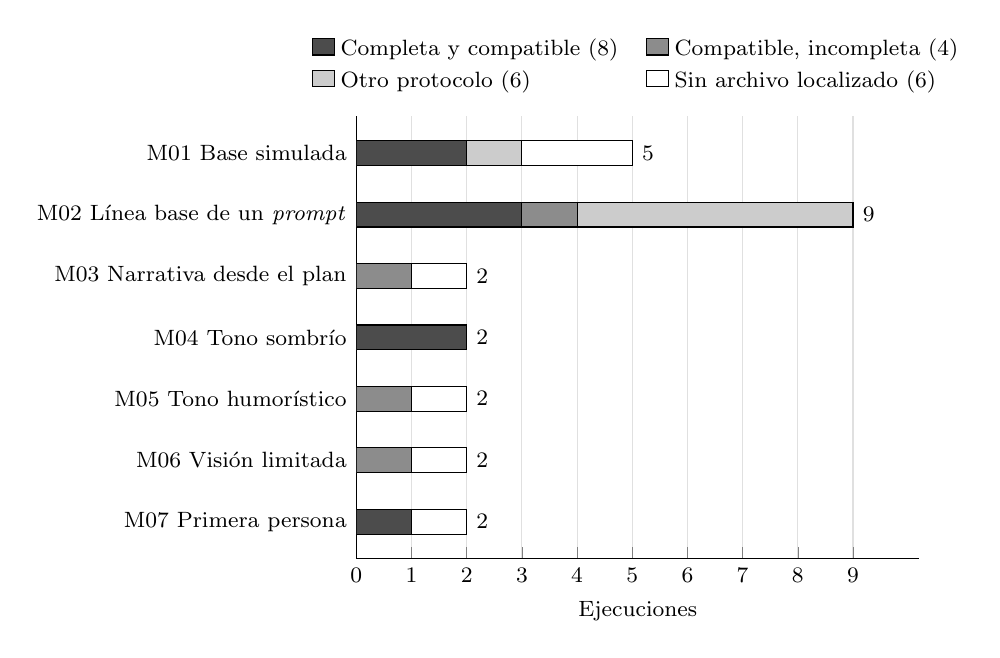
\begin{tikzpicture}
  \begin{axis}[
      xbar stacked,
      width=0.72\textwidth,
      height=7.2cm,
      bar width=9pt,
      font=\footnotesize,
      xmin=0, xmax=10.2,
      xtick={0,1,...,9},
      xlabel={Ejecuciones},
      ytick={1,...,7},
      yticklabels={
        M01 Base simulada,
        M02 Línea base de un \textit{prompt},
        M03 Narrativa desde el plan,
        M04 Tono sombrío,
        M05 Tono humorístico,
        M06 Visión limitada,
        M07 Primera persona},
      y dir=reverse,
      ymin=0.4, ymax=7.6,
      axis x line*=bottom,
      axis y line*=left,
      xmajorgrids,
      major grid style={draw=black!12},
      tick style={draw=black!50},
      legend style={at={(0.5,1.03)}, anchor=south, legend columns=2, draw=none,
        font=\footnotesize, /tikz/every even column/.append style={column sep=8pt}},
      legend cell align=left,
    ]
    \addplot[fill=black!70, draw=black] coordinates
      {(2,1) (3,2) (0,3) (2,4) (0,5) (0,6) (1,7)};
    \addplot[fill=black!45, draw=black] coordinates
      {(0,1) (1,2) (1,3) (0,4) (1,5) (1,6) (0,7)};
    \addplot[fill=black!20, draw=black] coordinates
      {(1,1) (5,2) (0,3) (0,4) (0,5) (0,6) (0,7)};
    \addplot[fill=white, draw=black] coordinates
      {(2,1) (0,2) (1,3) (0,4) (1,5) (1,6) (1,7)};
    \legend{Completa y compatible (8), {Compatible, incompleta (4)},
      Otro protocolo (6), Sin archivo localizado (6)}
    % Total de ejecuciones de cada celda, al final de su barra.
    \node[anchor=west] at (axis cs:5,1) {5};
    \node[anchor=west] at (axis cs:9,2) {9};
    \node[anchor=west] at (axis cs:2,3) {2};
    \node[anchor=west] at (axis cs:2,4) {2};
    \node[anchor=west] at (axis cs:2,5) {2};
    \node[anchor=west] at (axis cs:2,6) {2};
    \node[anchor=west] at (axis cs:2,7) {2};
  \end{axis}
\end{tikzpicture}

  \caption{Extracción núcleo de las 24 ejecuciones, por celda (2026-11-07)}
  \label{fig:horizontal}
\end{figure}

Como ejemplo del procedimiento se conserva el análisis de las cinco variantes de la primera base
de la obra 03. La Tabla~\ref{tab:piloto} presenta los tres rasgos calculados directamente desde el
texto que resultaron comparables en el informe del 30 de octubre. Las diferencias corresponden a un
par por variante y no estiman el ruido entre repeticiones del conjunto completo.

\begin{table}[htb]
  \centering
  \caption{Diferencias con la base de la obra 03 (un par por variante, 2026-10-30)}
  \label{tab:piloto}
  \footnotesize
  \setlength{\tabcolsep}{4pt}
  \begin{tabular}{@{}lrrrl@{}}
\toprule
Celda & Palabras & Proporción de diálogo & Repetición de trigramas & Lectura \\
\midrule
Base (valores absolutos) & 1.560 & 0,40 & 0,12 & --- \\
Narrativa desde el plan & $-$176 & $+$0,06 & $-$0,04 & n insuficiente \\
Tono sombrío & $-$80 & $+$0,02 & $-$0,05 & n insuficiente \\
Tono humorístico & $-$75 & $-$0,08 & $-$0,04 & n insuficiente \\
Visión limitada & $-$311 & $-$0,05 & $-$0,04 & n insuficiente \\
Primera persona & $-$157 & $-$0,02 & $-$0,06 & n insuficiente \\
\bottomrule
\end{tabular}

\end{table}

El contraste entre simulación y escritura directa dispone de dos ejecuciones narrativas vinculadas
a sus planes fuente. Para interpretar la magnitud de sus diferencias según la regla de la
Sección~\ref{sec:horizontal}, deben acompañarse de las extracciones compatibles y del ruido entre
repeticiones. El autor comunica que se midió ese ruido con un resultado favorable, pero el informe
numérico correspondiente no está identificado en los registros revisados; no se le asigna un valor
ni se extiende a las 24 ejecuciones el resultado del ejemplo de la obra 03.

\section{El estudio humano}\label{sec:resultados-estudio}

Según la información del autor actualizada el 7 de noviembre de 2026, participaron
\textbf{ocho lectores}, incluido el propio autor, durante octubre y hasta el 1 de noviembre.
Se seleccionaron por conveniencia entre colegas graduados de Ciencia de la Computación. Tres
indicaron frecuencia de lectura alta, tres media y dos baja. Estas categorías describen hábitos
de lectura; no proceden de una escala validada ni representan diversidad de formación académica.
La Tabla~\ref{tab:lectores} del Anexo~\ref{app:lectores} recoge los perfiles anónimos.

Todos leyeron los mismos \textbf{diez textos distintos}, distribuidos en \textbf{cinco pares},
mediante el bot de Telegram. El método que produjo cada texto permaneció oculto durante la
comparación; conocer que las historias eran generadas no revelaba qué configuración correspondía
a A o B. El autor conocía el funcionamiento del sistema y se identifica como participante para
separar sus respuestas en el análisis. Los pares se presentaron en el mismo orden; el registro
actualizado no precisa si la posición A/B se mantuvo o se alternó entre lectores.

En cada par se respondieron las tres preguntas de la Tabla~\ref{tab:criterios}: creatividad,
desarrollo de personajes e interés de la trama. Los botones ofrecían «Historia A», «Historia B» y
«No puedo decidir»; la última opción se registra como abstención y no distingue entre empate y
falta de una preferencia. El autor confirma que los ocho completaron las preguntas. La
Tabla~\ref{tab:participacion} expresa la participación resultante: 40 comparaciones lector-par y
120 respuestas, incluidas las posibles abstenciones. Las tres respuestas sobre un par no constituyen
tres comparaciones independientes.

\begin{table}[htb]
  \centering
  \caption{Participación declarada del estudio (octubre--1 de noviembre de 2026)}
  \label{tab:participacion}
  \small
  % Revisión documental 2026-11-07; fuentes en revision.json.
\begin{tabular}{@{}lr@{}}
\toprule
Magnitud & Cantidad \\
\midrule
Participantes (incluido el autor) & 8 \\
Textos distintos & 10 \\
Pares comunes & 5 \\
Comparaciones lector-par & 40 \\
Respuestas por criterio & 40 \\
Respuestas totales (incluyen abstenciones) & 120 \\
\bottomrule
\end{tabular}

\end{table}

Las respuestas se transcribieron manualmente a partir de la actividad del bot. El registro
individual del conjunto de ocho lectores y la correspondencia entre sus diez textos y los
identificadores de ejecución no se han localizado en los archivos disponibles para esta revisión.
Por ello, se informa la participación declarada, pero no se reconstruyen elecciones individuales,
porcentajes de preferencia ni coeficientes de acuerdo. Las salidas conservadas de un piloto anterior,
con cinco lectores y seis textos, tienen otro alcance y no se utilizan como resultados de este
estudio. Sus identificadores de lector tampoco se equiparan con los del anexo actual.

Cinco pares disjuntos sobre diez textos forman cinco componentes en el grafo de comparaciones.
Incluso con todas las respuestas, esos pares permiten estudiar preferencias dentro de cada pareja,
pero no identificar un orden humano global mediante Bradley-Terry. Las lecturas adicionales,
realizadas por algunos de los mismos participantes, podrían aportar conexiones si se documentan sus
pares; no se presupone que lo hagan ni se incluyen en las 120 respuestas principales.

La muestra permite describir una aplicación de la metodología con distintos hábitos de lectura.
Para estimar preferencias y su incertidumbre se necesita recuperar las respuestas por par y criterio,
separar las del autor y remuestrear por lector, como prevé la Sección~\ref{sec:agregacion}.
Ampliar la muestra y diversificar su formación permitirá estudiar cuánto se reproducen los resultados.

\section{El juez aprendido}\label{sec:resultados-juez}

El juez relaciona los rasgos del texto con las preferencias humanas mediante la regresión por pares
de la Sección~\ref{sec:juez}. Deben distinguirse las historias que aportan votos al entrenamiento,
las reservadas para validación y el corpus al que después se aplica el modelo. El autor sitúa el
análisis actualizado el 1 de noviembre de 2026, con respuestas de ocho lectores, y comunica un rango
de acierto de \textbf{0,50 a 0,65}. La Tabla~\ref{tab:juez-actual} precisa el alcance documental de
ese resultado.

\begin{table}[htb]
  \centering
  \caption{Resultado comunicado del juez y alcance de su documentación}
  \label{tab:juez-actual}
  \small
  % Revisión documental 2026-11-07; fuentes en revision.json.
\begin{tabular}{@{}>{\raggedright\arraybackslash}p{5.2cm}>{\raggedright\arraybackslash}p{8.2cm}@{}}
\toprule
Dato & Alcance disponible \\
\midrule
Acierto comunicado & 0,50--0,65; sin desglose por criterio ni partición \\
Fecha comunicada & 1 de noviembre de 2026 \\
Procedencia & Declaración del autor, revisada el 7 de noviembre \\
Validación fuera de muestra & Modalidad y denominadores pendientes de documentar \\
Control de longitud & Sin resultado actualizado localizado \\
\bottomrule
\end{tabular}

\end{table}

No se dispone del desglose por criterio, los denominadores ni la partición que produjo ese rango.
Por tanto, no se presenta como una medida verificada fuera de muestra ni se compara con los
porcentajes de longitud sola del piloto anterior. Tampoco se calculan intervalos o significación a
partir de sus extremos. El informe del juez conservado del 3 de noviembre corresponde al piloto de
cinco lectores; sus predicciones y perturbaciones permanecen como resultados históricos separados.

La evaluación del juez debe conservar las predicciones de cada partición y el control de longitud
sobre los mismos votos. La interpretación requiere considerar la dependencia entre respuestas de
un lector y la falta de un ranking humano global en los cinco pares principales. Un rango de
acierto, por sí solo, no establece que el modelo generalice a nuevas historias o lectores.

\section{La ordenación del corpus}\label{sec:resultados-ranking}

El corpus destinado a la ordenación comprende \textbf{122 historias}, según la actualización del
autor. Este número describe los textos a los que se quiere aplicar el juez; no es el tamaño del
conjunto de entrenamiento ni demuestra que todos tengan extracción compatible o puntuación.
La lista de identificadores y la salida de ordenación correspondiente siguen pendientes de
incorporación al registro reproducible.

Los archivos históricos del 3 de noviembre describen otro alcance: nueve historias ordenadas de un
inventario de 130 elegibles, con seis textos del entrenamiento del piloto. Se conservan con su fecha
y sus fuentes, pero sus puestos y perfiles no se trasladan al corpus actualizado de 122 historias.
Sin la lista y las puntuaciones de este último no se seleccionan diez títulos ni se atribuyen a sus
primeras posiciones los rasgos de las historias del informe anterior.

Para interpretar la ordenación deben identificarse la versión del juez, las extracciones utilizadas,
las exclusiones y la pertenencia de cada texto al entrenamiento. La lectura de las primeras historias
ha de relacionar sus rasgos con pasajes concretos, sin convertir la puntuación del modelo en una
medida absoluta de calidad (Sección~\ref{sec:ranking}).

\section{Respuesta a las hipótesis}\label{sec:respuesta-hipotesis}

Cada hipótesis se responde según el contraste que propone y el alcance de las observaciones:

\begin{itemize}
  \item \textbf{Simulación frente a escritura directa desde el mismo plan (H1).} La matriz conserva
  dos narrativas derivadas de planes de bases simuladas y un informe de diferencias textuales para
  la obra 03. La asociación de los cinco pares humanos con esos contrastes requiere identificar
  los diez textos del estudio. Se conserva el contraste mecánico documentado; la preferencia
  específica por la simulación y su relación con el ruido deben establecerse con los registros
  correspondientes y una muestra ampliada de lectores.
  \item \textbf{Memoria propia frente a memoria compartida (H2).} El autor informa de una comparación
  realizada con resultado favorable a la memoria propia. La auditoría documentada de 62 contextos
  muestra aislamiento de pensamientos y susurros, pero no cuantifica el contraste entre ambas
  configuraciones. Los tres intentos con memoria compartida localizados en la versión 7.9 terminaron
  con fallo y no identifican el experimento comunicado. Para expresar su magnitud se necesitan los
  pares de ejecuciones, los recuentos de menciones desconocidas y las preferencias; no se deducen
  esos valores de la configuración del sistema.
  \item \textbf{Mejora mecánica y preferencia humana (H3).} Las sesiones conservadas de narración
  y escritura muestran mejoras en las medidas de prosa sin una victoria del brazo modificado:
  empate en narración y preferencia por el brazo sin esos mecanismos en tres de cuatro pares de
  escritura. Es evidencia descriptiva compatible con que una mejora mecánica no garantiza una
  preferencia humana. Las lecturas adicionales comunicadas deben documentarse para extender el
  alcance de esta observación; un empate o una diferencia no significativa no demuestran
  equivalencia entre configuraciones.
\end{itemize}

El capítulo documenta una configuración de referencia, 24 ejecuciones para el análisis horizontal y
un estudio de ocho lectores con 120 respuestas declaradas. Los instrumentos permiten relacionar
rasgos, comparaciones y configuraciones; su interpretación exige mantener la correspondencia entre
cada cifra y su fuente. El rango de acierto comunicado del juez y el corpus de 122 historias se
presentan con ese alcance, mientras que la generalización de las preferencias requiere ampliar la
muestra y completar su trazabilidad.
